\documentclass[../Head/Report.tex]{subfiles}
\begin{document}
\section{Introduction}
When processing big amount of data or jobs for which a large amount of resources are required, never computers often tend to be a pretty expensive solution. If the job does not have to be computed on a single unit, a distribution of the workload on multiple entities could be a possibility. If one got access to a supercomputer or another campus where multiple machines are accessible, this could effectively solve your problem.

This project presents a way to build a Raspberry Pi cluster where parallel computing of big data will be distributed to multiple nodes using SLURM. The compute nodes will share data on the master node by building a network file system (NFS). The computation of data will then be distributed to the compute nodes using OpenMPI where the code is written in python. The time for which the data has been processed and completed will be compared to that of a regular computer to see how fast a Pi cluster is able to compute a big amount of data.

Four Raspberry Pi 2 will be used in the cluster. This Raspberry Pi can be seen in Figure \ref{fig:raspberry_pi}. One of them will be a master and the rest slaves. A USB with a capacity of 128 GB will be used in the master for which file sharing will be utilized between the slaves.  

\begin{figure}[H]
\centering
  \begin{subfigure}[b]{0.48\textwidth}
  \centering
    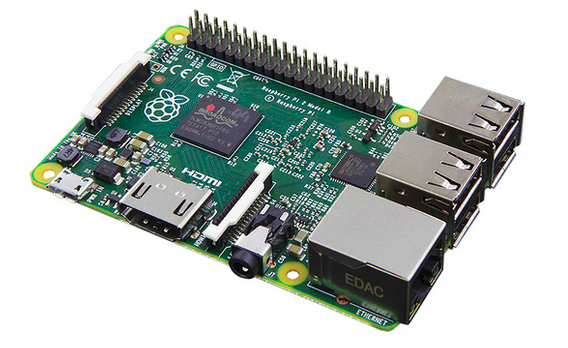
\includegraphics[height=5cm]{../Figures/raspberry_pi.png}
    \caption{Raspberry Pi 2}
    \label{fig:raspberry_pi}
  \end{subfigure}
  \hfill
  \begin{subfigure}[b]{0.48\textwidth}
  \centering
    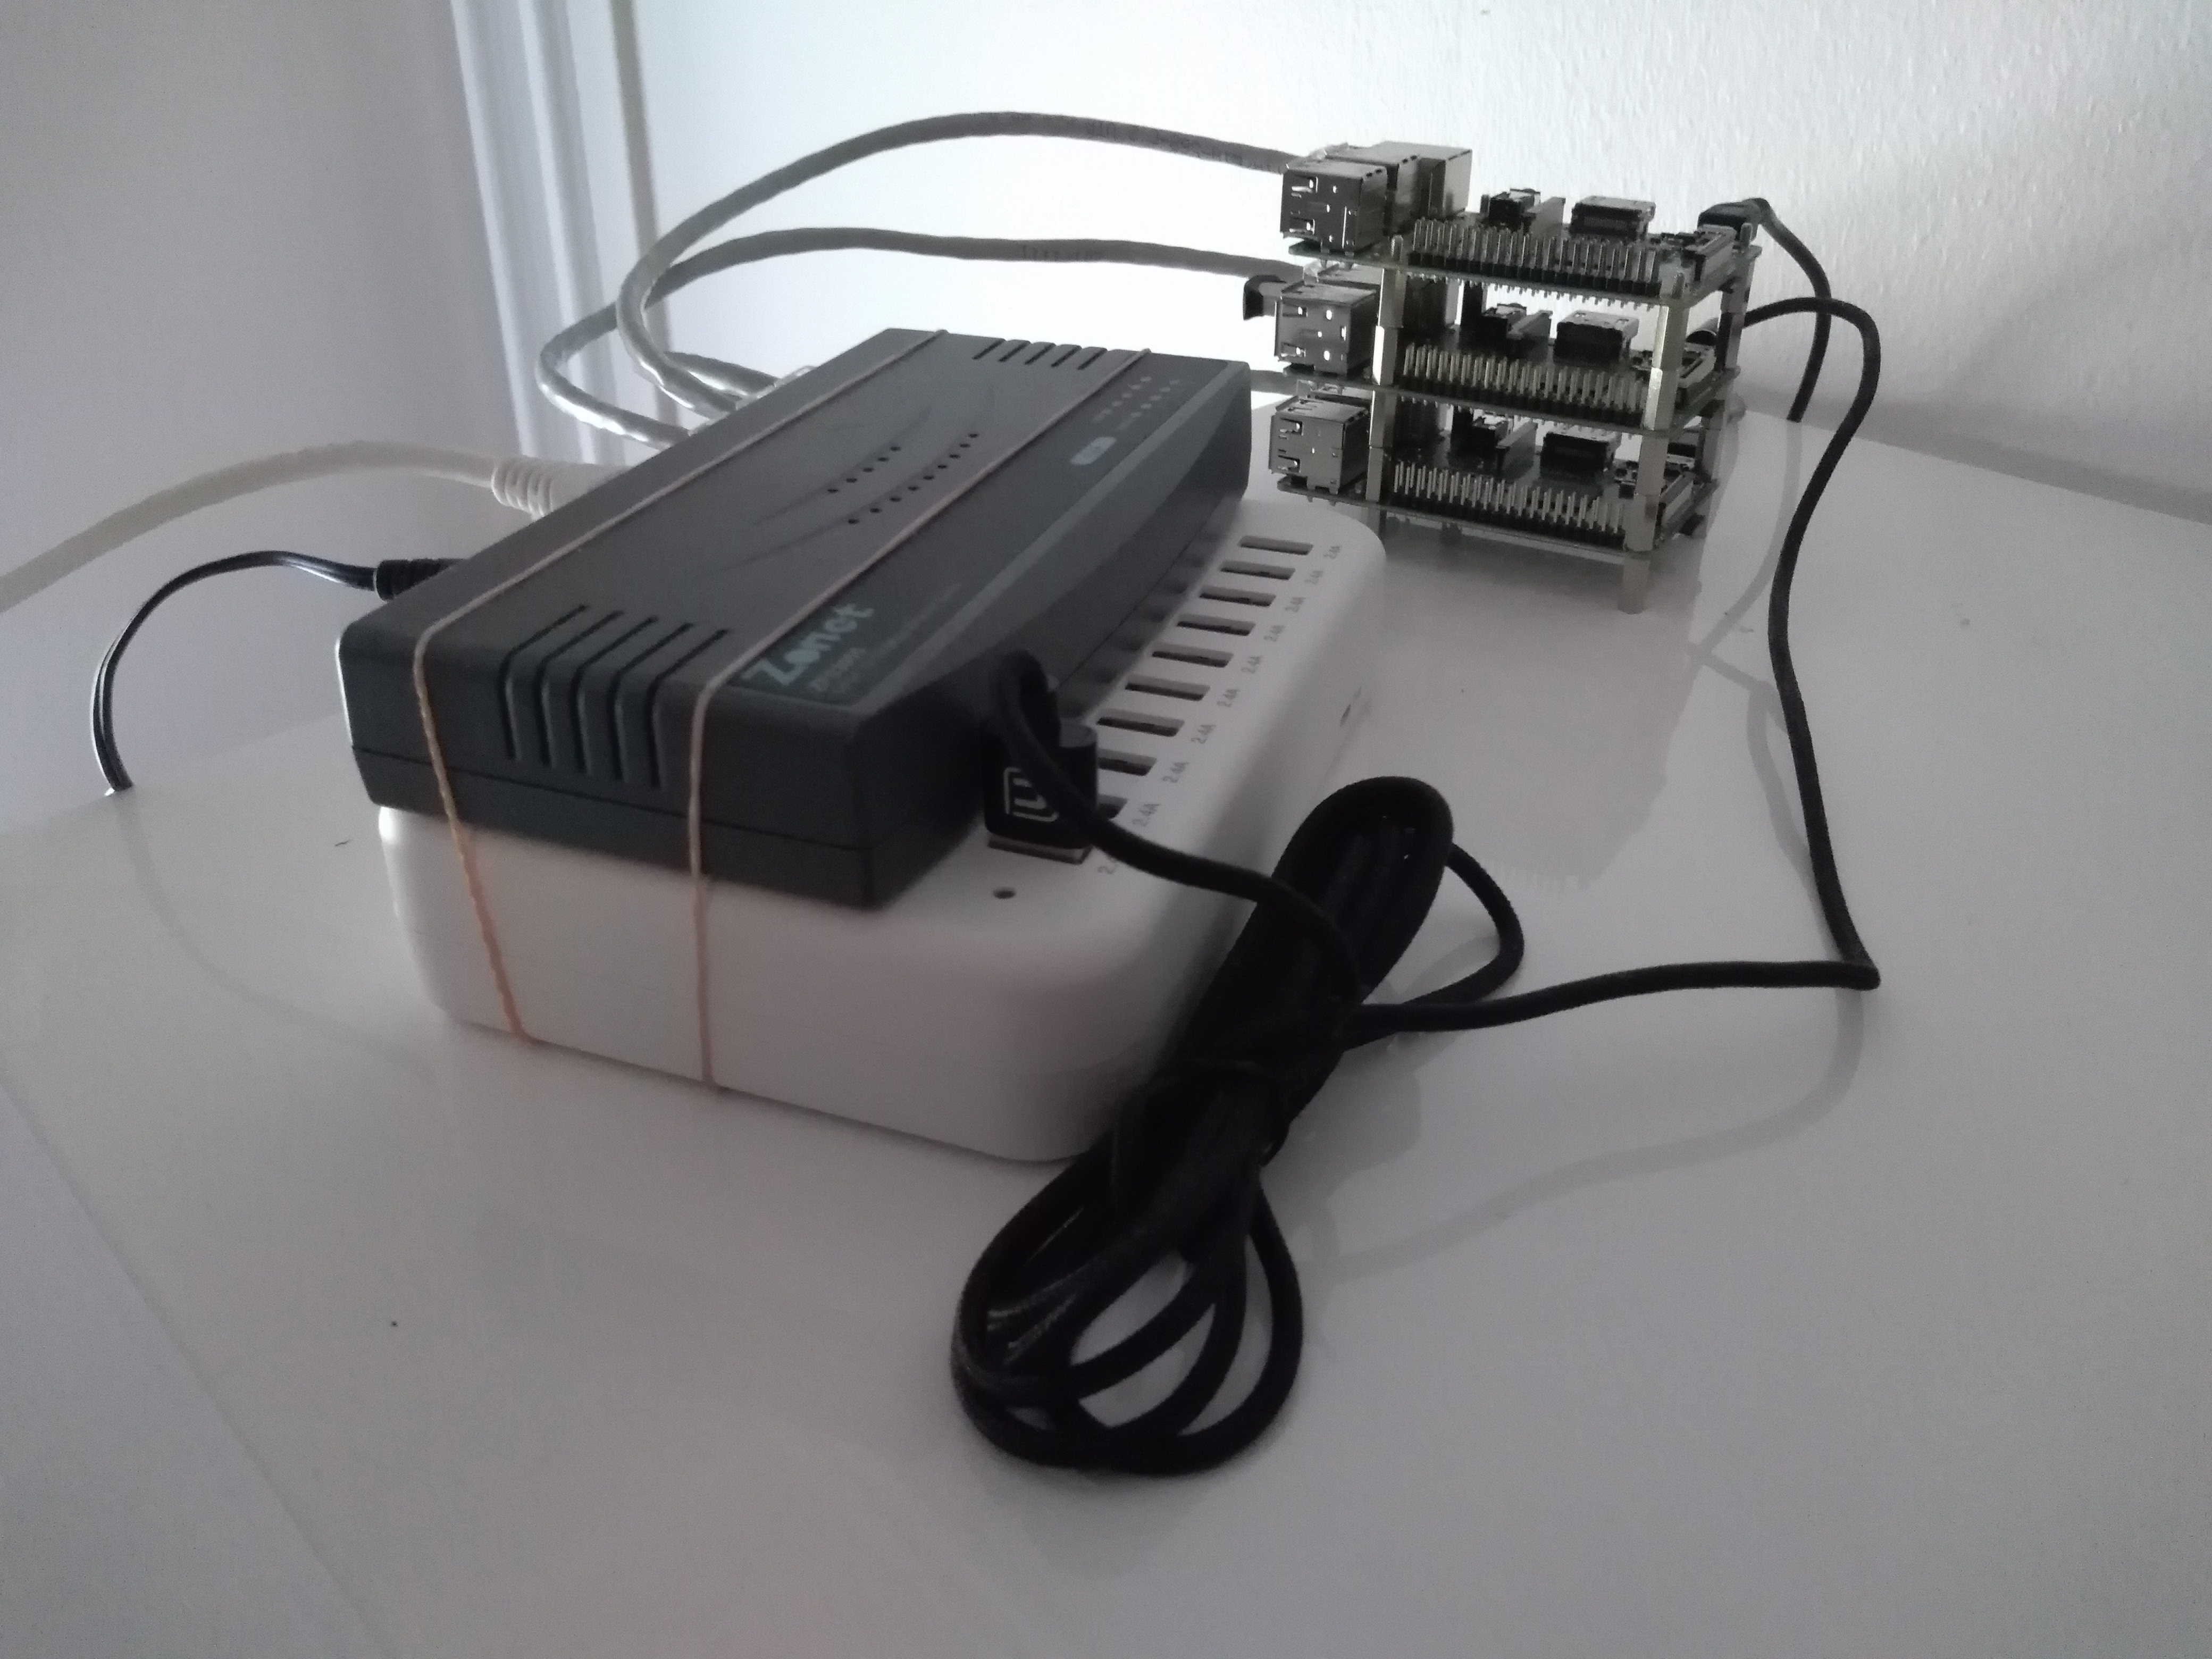
\includegraphics[height=5cm]{../Figures/cluster.jpg}
    \caption{The cluster, network switch and USB power hub}
    \label{fig:cluster}
  \end{subfigure}
  \caption{Illustration Raspberry Pi used along with the Raspberry Pi cluster }
\end{figure}
    
For communication between the nodes and the laptop, a network switch with five I/O will be used. A USB hub will also be present as an alternative power supply for the cluster if needed. Furthermore, four MicroSD cards will be used to store the Raspbian Buster Lite image used to run the nodes.  

The following chapters will cover the setup of the Raspberry Pi cluster along with testing of the distribution of data between the nodes.   

\section{Raspberry Pi setup}
The Raspbian Buster Lite operating system will be used on the nodes in order to minimize software as this is appropriate to solve the task. To flash the image to the Raspberry Pi \textit{balenaEtcher} is used. After this operation, an empty file called \textit{ssh} is created in the boot drive of the MicroSD card in order to enable secure shell (SSH) as the communication between the Raspberry Pi and laptop. Now using \textbf{ssh pi@raspberrypi.local} from the laptop a communication is established. It is important that the default password will be changed which is \textit{raspberry}. To do this, enter \textbf{raspi\_confic} and follow the instructions. In the \textit{raspi\_config} menu, it is also possible to allocated all memory to the operating system in the \textit{advanced options} and hence expand \textit{files system}.   

As a preparation to using SLURM, the hostname is changed to \textit{node01} for the hostname and in the files /etc/hostname and /etc/hosts using \textbf{sudo hostname node01}, \textbf{sudo nano /etc/hostname} and \textbf{sudo nano /etc/hosts} respectively. This is done for the master (node01) and the slaves with numbers going from 2-4. Nano is the default command line text editor along with vi.  

\subsection{Mount flash drive}
The external storage which is going to be used as shared memory between nodes in the cluster, will be installed on the master (node01). 

Using the command \textbf{lsblk}, a list of drives on the Raspberry Pi are listed in the terminal. In this case, the drive /dev/sda1 is the wanted USB. The drive is now formatted using \textbf{sudo mkfs.ext4 /dev/sda1}. The next step is to create a directory where the shared folder should be placed. This is done with \textbf{sudo mkdir /clusterfs}, \textbf{sudo chown nobody.nogroup -R /clusterfs} and \textbf{sudo chmod 777 -R /clusterfs} for making the directory, changing the ownership and read-write permissions respectively. 

Each file system gets assigned a universally unique identifier (UUID) during formatting. Since it cannot be changed, it is an ideal way to select file systems for mounting \cite{fstab}. To setup automatic mounting, this UUID for the flash drive must be known which can be found using \textbf{blkid}. Now the line \textit{UUID="7e098cc9-23f9-4226-a73e-6fdeed70bd83" /clusterfs ext4 defaults 0 2} can be added in the file /etc/fstab. Here the chosen directory is selected along with file type and fifth field with a 2 indicating that it is not a root file system \cite{fstab_pass}. To mount the drive, \textbf{sudo mount -a} can be used or just reboot the Pi. 

\subsection{Networking}
The Raspberry Pis must have access to the internet. This is accomplished by setting up a shared network where the Pis will use the network from the laptop with a connection named \textit{Cluster} which is made using \textit{nm-connection-editor} in the IPv4 settings where \textit{shared to other users} are chosen. 

First the laptop is setup for the shared network. A file called rc.nat is created in /etc/rc.d directory. Here the lines \textit{(iptables=/sbin/iptables)}, which specifies the location of the iptables executables, \textit{(iptables --flush -t nat)}, which clears iptables rules, \textit{(iptables --table nat --append POSTROUTING --out-interface ppp0 -j MASQUERADE)} and \textit{(iptables --append FORWARD --in-interface eth0 -j ACCEPT)}, for setting network address translation (NAT) and forwarding of packages and then \textit{(echo 1 > /proc/sys/net/ipv4/ip\_forward)} for enabling of packet forwarding, will be added to the file. Now make this file executable and it will executed every time the computer is started \cite{Networking}.

To make the setup of each Raspberry Pi more systematic, the interface name for each Pi is changed to a constant value, namely \textit{etc0}. This is done finding the MAC address of each Pi during setup. Then adding the lines \textit{(ATTR{address}=="b8:27:} \textit{eb:11:5e:b0")} and \textit{(NAME="eth0")} to the file /etc/udev/rules.d/70-persistent-net.rules and adding the lines \textit{(DEVICE=} \textit{"eth0")} and \textit{(HWADDR="b8:27:eb:11:5e:b0")} to the file  \textit{/etc/sysconfig/network-scripts/ifcfg-eth0}. The master node is used as a description of the implementation for which its MAC address is used. This must of cause be changed accordingly to the other nodes.\cite{Interface_Name}     

In the Raspberry Pi, a static IP address is setup by adding the lines \textit{(interface eth0)}, \textit{(static ip\_address=10.42.0.10/24)}, \textit{(static routers=10.42.0.1)} and \textit{(static domain\_name\_servers=10.24.0.1)} to the file /etc/dhcpcd.conf (there is no specific reason for choosing the mentioned IP address). Because this IP address it set for the master node, the slaves will have there last byte going from 11-13.

\subsection{Network file system (NFS)} 

NFS is a program used to share files and folders between Linux/unix systems and hence an optimal chose for this project. The mounted drive (USB) on the master node must be exported as a network file system. This enables the other nodes on the network to get access to it. 

The NFS server is installed on the master node using \textbf{sudo apt install nfs-kernel-server}. By adding the line \textit{(/home/pi/clusterfs 10.42.0.0/24(rw,sync no,root\_squash no,no\_subtree\_check)} to the file /etc/export, the content of the given directory is exported to the remote hosts. The parameters gives read-write permission, forced changes to be written on each transaction, enables the root users of clients write files with root permissions and prevention of error if race condition occurs during read-write of files. The kernel server can now be updated using \textbf{sudo exportfs -a}. 

Now the NFS client must be installed on the slave nodes which is done using the command \textbf{sudo apt install nfs-common}. Then a shared folder can be made using \textbf{sudo mkdir /clusterfs} with owner and permissions changed using \textbf{sudo chown nobody.nogroup} \textbf{/clusterfs} and \textbf{sudo chmod -R 777 /clusterfs}. To make the NFS share to mount automtically when nodes boot, the /etc/fstab file should be changed with the line \textit{(10.42.0.10:/home/pi/clusterfs /home/pi/clusterfs nfs defaults 0 0)}. This sets the file system, mount point, type, options, dump and pass. \cite{NFS}

\section{Slurm}

Simple Linux Utility for Resource Management (SLURM) is an open source highly scalable cluster management and job scheduling system for large and small Linux clusters. It can allocate access to resources for users for a duration of time so they can perform work. Moreover, it provides framework for starting , executing and monitoring work on allocated nodes along with an arbitration contention for resources by managing a queue of pending work. Hence this software is chosen for management of the Raspberry Pi cluster. Fore more information visit \cite{SLURM}. 

First the master node is going to be configured. As already mentioned, the Raspberry Pi with IP address 10.42.0.10 (Node01) will be the master. To make access to the units in our cluster easier, the line \textit{(10.42.0.11 node02)} is added to the file /etc/hosts for every Pi connected to our cluster where the the IP address will go from 11-13 and node from 2-4. Then the SLURM controller packages will be installed using \textbf{sudo apt install slurm-wlm}. In order to initiate SLURM with defaults configurations, the file slurm.conf.simple is fetched to /etc/slurm-llnl using \textbf{cp /usr/share/doc/slurm-client/examples/slur} \textbf{m.conf.simple.gz .} Now unzip the file \textbf{gzip -d slurm.conf.simple.gz} and renaming it to slurm.conf, we can make changes to the configurations which fits our needs. The control machine (master) have to spefified in the this file with the line \textit{ SlurmctldHost=node01(10.42.0.10)}. Now in the bottom of the file, all the nodes in the cluster have to be specified with the line \textit{(NodeName=node01 NodeAddr=10.42.0.10 CPUs=4 State=UNKNOWN)}. Again the nodes will go from 1-4 and the last byte of the IP address from 10-13. This is done so that SLURM knows all the units and the amount of resources in the cluster. SLURM runs of partitions for which nodes can be given. Two lines with a partition name along with the avalible nodes will be added as \textit{PartitionName=mycluster1 Nodes=node[02-04] Default=YES} and \textit{MaxTime=INFINITE State=UP}. The nodes given will be the compute nodes of the cluster. It is important that this file is consistent across all nodes in the cluster.    

The way to restrict access to system resources is to create and modify the cgroup.conf file which will be utilized in the directory \textit{/etc/slurm-llnl/}. This will limit the amount of resources SLURM gives to each job. The configurations can be seen to the left in Figure \ref{fig:created_files}.     

\begin{figure}[H]
	\centering
	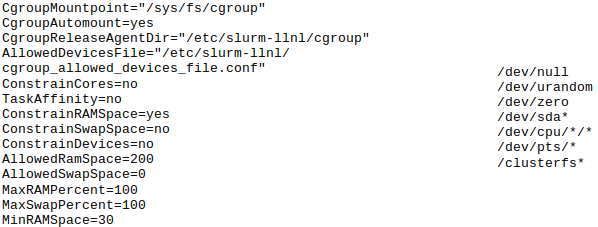
\includegraphics[height=5cm]{../Figures/created_files.png}
    \caption{Configuration of cgroup.conf and cgroup\_allowed\_devices\_file.conf respectively}
    \label{fig:created_files}
\end{figure}

The \textit{CgroupAutomount} is set to yes so that the plugin will first try to mount the required subsystems. If not set, if will fail if they are not available. The \textit{CgroupMountpoint} defines the path under which cgroups should be mounted. The \textit{AllowedDevicesFile} specifies devices to use which is configured in the file \textit{cgroup\_allowed\_devices\_file.conf} that can be seen to the right in Figure \ref{fig:created_files}. The rest of the lines primarily specifies minimum, maximum and permission to use cores and memory of the system. \cite{cgroups} \cite{piCluster}. 

Munge is used as the default authentication mechanism in SLURM which is similar to key-based SSH. It will use a private key across all nodes, then requests are timestamp-encrypted and sent to the nodes that encrypts them using the identical key. For this to work, the time across all nodes must be synchronized. This is accomplished by installing \textit{ntpdate} on all nodes using \textbf{sudo apt install ntpdate}. 

Now the files slurm.conf cgroup.conf cgroup\_allowed\_devices\_file.conf is copied to the /clusterfs directory using \textbf{sudo cp slurm.conf cgroup.conf cgroup\_allowed\_devices\_file.conf /clusterfs}. Also the munge key will be copied to this directory as \textbf{sudo cp /etc/munge/munge.key /clusterfs}. This is done so that the configuration file is the same across all nodes so that they can be controlled by SLURM. Now we can start Munge, the SLURM daemon and control daemon using \textbf{sudo systemctl enable munge}, \textbf{sudo systemctl start munge}, \textbf{sudo systemctl enable slurmd}, \textbf{sudo systemctl start slurmd}, \textbf{sudo systemctl enable slurmctld} and \textbf{sudo systemctl start slurmctld} respectively.

Now on all the compute notes the slurmd and slurm-client must be installed using \textbf{sudo apt install slurmd slurm-client}. Like with the master node, the IP address and node name will be added to the file /etc/hosts of all the other nodes in the cluster. Moreover, the munge.key, slurm.conf and cgroup files from the created /clusterfs directory will be copied to each node using \textbf{sudo cp /clusterfs/munge.key /etc/munge/munge.key}, \textbf{sudo cp /clusterfs/slurm.conf /etc/slurm-llnl/slurm.conf} and \textbf{sudo cp /clusterfs/cgroup* /etc/slurm-llnl}. This way we can be sure that we have the same configuration files and Munge key across all the nodes in the cluster. Now we just have to enable and start Munge and the SLURM daemon using \textbf{sudo systemctl enable munge}, \textbf{sudo systemctl start munge}, \textbf{sudo systemctl enable slurmd} and \textbf{sudo systemctl start slurmd} respectively.

\section{Big data processing}

OpenMPI is an open source message passing interface which enables a single script to run a job spread across multiple nodes in the cluster. To use OpenMPI, the following must be installed on every node \textbf{sudo apt install openmpi-bin openmpi-common libopenmpi3 libopenmpi-dev}.

Because the most time consuming operation in the cluster is the communication and sharing of data between nodes, two programs will be tested. A program of computing an integral running locally on each node will performed. Moreover, a program for counting pumpkins in a field where sharing of the data will happen from the USB of the master will also be utilized.    

\definecolor{backcolour}{rgb}{0.95,0.95,0.92}

\lstset{ 
backgroundcolor=\color{white},
frame=none,
backgroundcolor=\color{backcolour}
}

\begin{figure}[H]
\centering
\begin{minipage}{0.9\textwidth}
\lstinputlisting[language=Python]{../../runtime_calculations/cal_pumpkins.py}
\end{minipage}
\caption{The code in the script cal\_pumpkins.py for parallel processing using OpenMPI}
\label{fig:cal_pumpkins.py}
\end{figure}

\begin{figure}[H]
\centering
\begin{minipage}{0.9\textwidth}
\lstinputlisting[language=bash]{../../runtime_calculations/sub_mpi_pumpkins.sh}
\end{minipage}
\caption{The code in the script sub\_mpi\_pumpkins.sh for parallel processing using OpenMPI and SLURM}
\label{fig:cal_pumpkins.py}
\end{figure}

\begin{figure}[H]
\centering
  \begin{subfigure}[b]{0.48\textwidth}
  \centering
    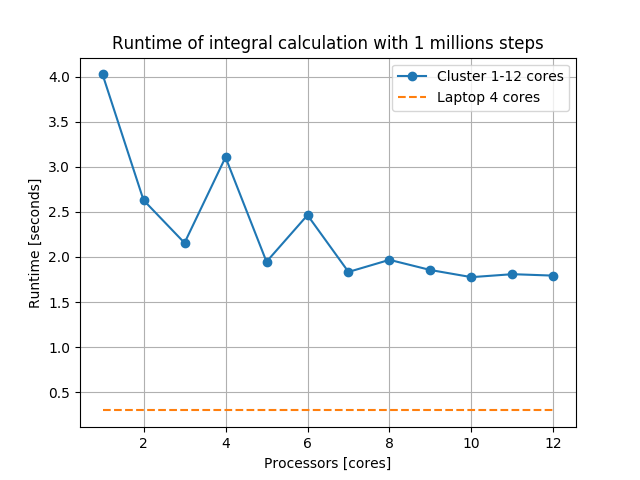
\includegraphics[height=6cm]{../Figures/integral_runtime_test_1mio.png}
    \caption{Runtime of an integral with 1 million steps}
    \label{fig:integral_runtime_1mio}
  \end{subfigure}
  \hfill
  \begin{subfigure}[b]{0.48\textwidth}
  \centering
    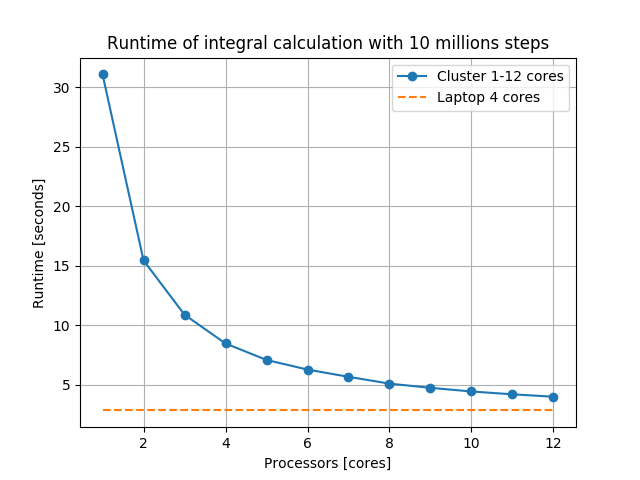
\includegraphics[height=6cm]{../Figures/integral_runtime_test_10mio.png}
    \caption{Runtime of an integral with 10 million steps}
    \label{fig:integral_runtime_10mio}
  \end{subfigure}
  \caption{The performance of a compute cluster in regard to a laptop}
\end{figure}

\begin{figure}[H]
\centering
\captionsetup{justification=centering}
  \begin{subfigure}[b]{0.48\textwidth}
  \centering
    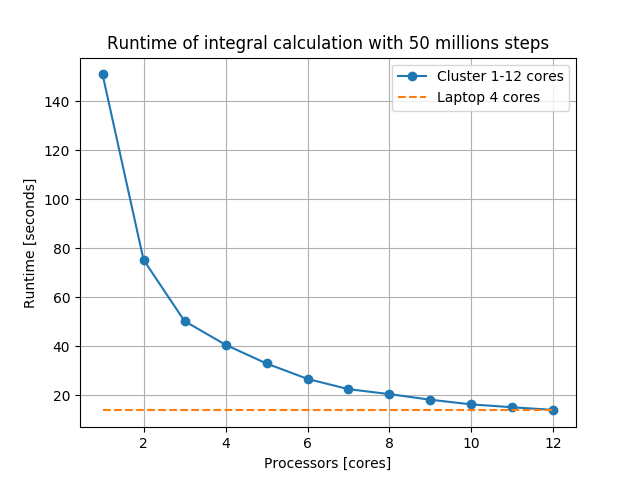
\includegraphics[height=6cm]{../Figures/integral_runtime_test_50mio.png}
    \caption{Runtime of an integral with 50 million steps}
    \label{fig:integral_runtime_50mio}
  \end{subfigure}
  \hfill
  \begin{subfigure}[b]{0.48\textwidth}
  \centering
    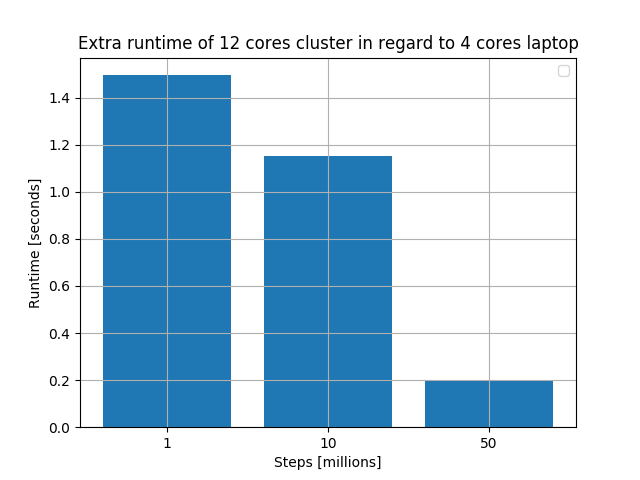
\includegraphics[height=6cm]{../Figures/barchart_runtime.png}
    \caption{Runtime of an integral with 10 million steps}
    \label{fig:extra_runtime_cluster}
  \end{subfigure}
  \caption{The performance of a compute cluster in regard to a laptop and the extra run time for the compute cluster summarized in a bar chart}
\end{figure}

\begin{figure}[H]
	\centering
	\captionsetup{justification=centering}
	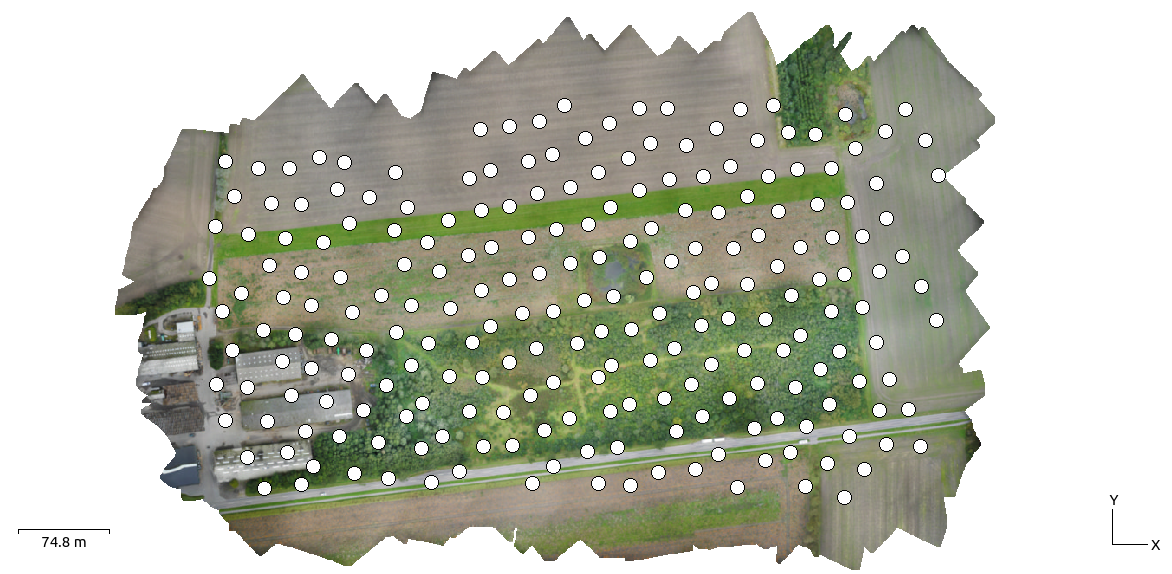
\includegraphics[height=7cm]{../Figures/orthomosaic.png}
    \caption{Illustration of the field in which pumpkins must be found. This is an orthomosaic made by the program Metashape from Agisoft}
    \label{fig:created_files}
\end{figure}

\begin{figure}[H]
	\centering
	\captionsetup{justification=centering}
	\includegraphics[height=17cm]{../Figures/big_data_handling.png}
    \caption{Illustration of the working of the pumpkin counting algorithm. The colors shows pumpkins detected in each block with an overlap to insure that pumpkins are only counted ones for each block}
    \label{fig:created_files}
\end{figure}

\begin{figure}[H]
\centering
  \begin{subfigure}[b]{0.48\textwidth}
  \centering
    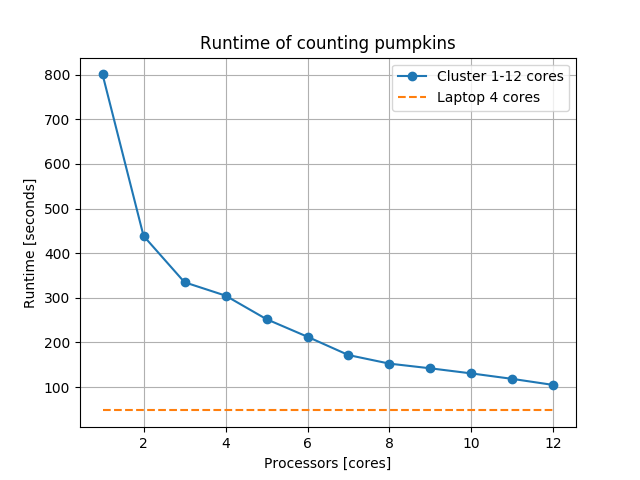
\includegraphics[height=6cm]{../Figures/runtime_counting_pumpkins1.png}
    \caption{Runtime of an integral with 1 million steps}
    \label{fig:integral_runtime_1mio}
  \end{subfigure}
  \hfill
  \begin{subfigure}[b]{0.48\textwidth}
  \centering
    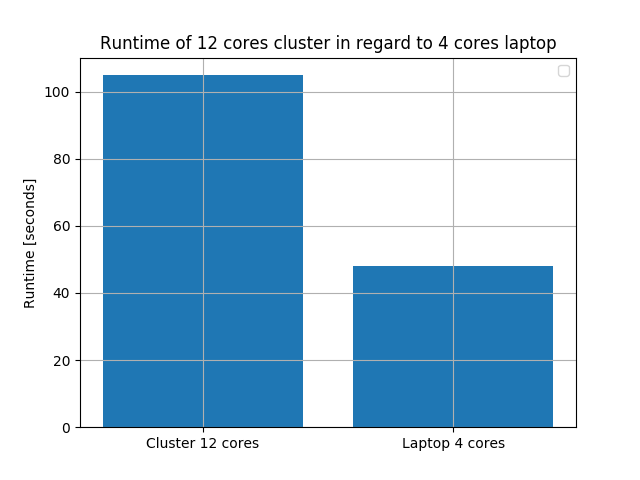
\includegraphics[height=6cm]{../Figures/barchart_pumpkin_runtime.png}
    \caption{Runtime of an integral with 10 million steps}
    \label{fig:integral_runtime_10mio}
  \end{subfigure}
  \caption{The performance of a compute cluster in regard to a laptop}
\end{figure}

\section{Discussion}
\section{Conclusion}





\end{document}